\chapter{Regeln und Regelmengen}

Im Folgenden werden konkrete Regelmengen vorgestellt, die zur Transformation von Plänen genutzt werden. Zuerst werden die Regelmengen von Pellenkoft vorgestellt. Die Regelmenge wurde von \cite{shanbhag2014optimizing} als unvollständig kritisiert. Dieser Kritik wird in einem weiteren Teil nachgegangen. Außerdem wird die Implementierung einer neuen Regel, ebenfalls von \cite{shanbhag2014optimizing} erörtert. 


\section{Pellenkoft Rulsets}

Bei der Erforschung eines Search Spaces kommen in regelbasierten \ac{QO} Transformationsregeln zum Einsatz. Pellenkoft et al. \cite{pellenkoft1997duplicate} \cite{manegold2000multi} \cite{pellenkoft1997complexity} stellt drei Regelsets zur Verfügung, die bei der Erzeugung eines Search Spaces zum Einsatz kommen können.



Zu Beginn besteht ein Search Space aus einem Plan. Dieser Plan stellt die Eingabe dar. Auf ihn werden Transformationsregeln angewendet. Neue Pläne entstehen. Sollten diese Pläne noch nicht vorhanden sein, werden sie dem Suchraum hinzugefügt. Pläne auf die bereits alle anwendbaren Transformationsregeln angewendet wurden, werden als besuchte Pläne bezeichnet. Sobald alle Pläne besucht wurden und somit auf alle Pläne Transformationsregeln auf alle Pläne angewendet wurden, ist der Suchraum vollständig erforscht und keine weiteren Pläne können gefunden werden. Der Actual Search Space ist ausgeschöpft.

Mehrere Transformationsregeln werden gemeinsam als Regelsets bezeichnet. Pellenkoft et al. unterscheidet zwischen Regelsets, die Pläne mehrfach generieren können und Regelsets, die duplikatfrei sind. Beispielsweise kann durch die Anwendung der Regel Kommutativität auf einen Plan und erneute Anwendung auf dessen Resultat  der ursprüngliche Plan generiert werden. Im Folgenden werden zwei Regelsets vorgestellt, die Duplikate bilden und ein Regelset, das duplikatsfrei ist.


\subsection{Regelset mit Duplikaten}

Eines der Regelsets, das zur Erzeugung eines Bushy Tree Space genutzt werden kann, ist $RS-B0$. Es besteht aus drei Regeln:

\begin{itemize}
\item Kommutativität: $$ A \Join B \to B \Join A$$
\item Rechte Assoziativität: $$(A \Join B) \Join C \to A \Join (B \Join C) $$
\item Linke Assoziativität: $$A \Join (B \Join C) \to (A \Join B) \Join C$$
\end{itemize}

Das Regelset ist redundant, da mit Hilfe von Kommutativität und rechter Assoziativität linke Assoziatvität (und vis-à-vis) erzeugt werden kann. Möchte man die Redundanz vermeiden, lässt sich Regelset $RS-B1$ erstellen. Es basiert auf Kommutativität und einer Swap genannten Regel:

\begin{itemize}
\item Swap $$ (A \Join B) \Join C \to (A \Join C) \Join B $$
\item Bottom Commutativitity $$ B_1 \Join B_2 \to B_2 \Join B_1$$
\end{itemize}


<<<<<<< HEAD
Durch die Anwendung der Regeln aus $RS-B0$ und $RS-B1$ können Pläne doppelt erzeugt werden. Am einfachsten ist dies an Hand von Kommutativität zu zeigen. Wird auf den Plan $a \Join b$ Kommutativität angewendet, entsteht b JOIN a, dann entsteht durch  die erneute Anwendung von Kommutativität auf den neuen Plan B JOIN A wieder der ursprüngliche Plan.

Ebenfalls können sich bei komplexeren Plänen     Teilpläne gleichen. Beispielsweise enthält der Plan $(A \Join B) \Join C$ den gleichen Subplan wie $C \Join (A \Join B)$. Um solche Duplikate zu verhindern, wird von Pellenkoft das Prinzip der Äquivalenzklasse angewendet.
=======
Ebenfalls können sich bei komplexeren Plänen     Teilpläne gleichen. Beispielsweise enthält der Plan $(A \JOIN B) \JOIN C$ den gleichen Subplan wie $C \JOIN (A \JOIN B)$. Um solche Duplikate zu verhindern, wird von Pellenkoft das Prinzip der Äquivalenzklasse angewendet.
>>>>>>> 2dbe3382d95b975a93a2c2789dd91dda3468d5cc



\subsection{Duplikatfreie Regelsets}
Durch die Anwendung on $RS_B0$ bzw. $RS_B1$ ist es möglich, dass Varianten des Plans erneut erzeugt werden. Dieser Gefahr trägt das Regelset RS-B2 Rechnung. Es sieht vor, dass eine Regel nur genau einmal ausgeführt und andere Regeln nur einmal pro Operator ausgeführt werden dürfen. Dieses Regelset besteht aus:


\begin{itemize}
\item Kommutativität: $$ A \Join B \to B \Join A$$
\item Rechte Assoziativität: $$(A \Join B) \Join C \to A \Join (B \Join C) $$
\item Linke Assoziativität: $$A \Join (B \Join C) \to (A \Join B) \Join C$$

\item Exchange $$(A \Join B) \Join (C \Join D) \to (A \Join D) \Join (C \Join B) $$
\end{itemize}



\subsubsection{Kreuzproduktfreie Regelsets und Vollständigkeit}

Die bisherigen Regelsets können zu Kreuzprodukten führen. Ebenfalls ist nicht geklärt, ob die Regelsets vollständig sind und alle möglichen kreuzproduktfreien Bäume erzeugen. Im Folgenden wird zuerst der Begriff der Kreuzproduktfreiheit eingeführt und basierend auf diesem Begriff die Vollständigkeit erläutert.

Ein Kreuzprodukt kann bei den vorliegenden Plänen dann entstehen, wenn durch die Anwendung einer Regel ein Join zwischen zwei Relationen gebildet wird, die zuvor keine Kante auf einem gegeben Join Tree hatten.

Eine Technik um Kreuzproduktfreiheit bei den bisherigen Regelsets herzustellen, ist die Unterdrückung von Kreuzprodukten die auch als \ac{CPS} bezeichnet wird. Der Ansatz funktioniert so, dass eine Regel, falls sie ein Kreuzprodukt erzeugt zwar als ausgeführt markiert, jedoch nicht der Baum in den Search Space aufgenommen wird. Somit werden Kreuzprodukte zwar erzeugt, aber nicht in den Suchrraum aufgenommen. Regelsets, die diese Art von Kreuzproduktunterdrückung anwenden, erhalten das Suffix CPS. Somit entstehen aus den Regelsets RS-B0, RS-B1 und RS-B2 die Regelsets RS-B0-CPS, RS-B1-CPS und RS-B2-CPS.


Eine andere wichtige Eigenschaft von Regelsets ist Vollständigkeit. Sie setzt voraus, dass Kreuzproduktfreiheit gegeben ist. Vollständigkeit liegt dann vor, wenn alle kreuzproduktfreien Pläne in einem Suchraum erzeugt wurden.


<<<<<<< HEAD
=======
\subsubsection{Unvollständigkeit von RS-02}


\begin{figure}[h]
  \centering
  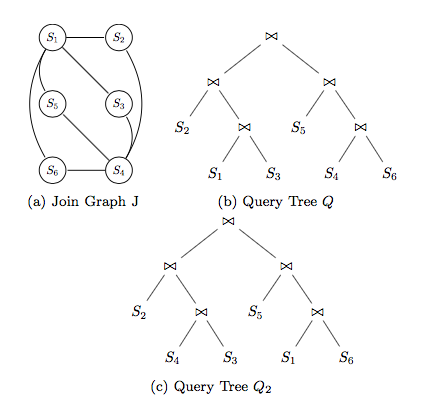
\includegraphics[width=\textwidth]{03_Related_Work/Incompleteness_RS-B2-CPS.png}
  \caption{Incompletness of RS-B2-CPS}
  \label{Incompleteness_RS-B2-CPS}
\end{figure}


\cite{shanbhag2014optimizing} stellt fest, dass RS-B0-CPS und RS-B1-CPS vollständig sind. Die Vollständigkeit von RS-B2-CPS wird jedoch in Frage gestellt und die Unvollständigkeit mit Hilfe eines Beispiels belegt. Als Beispiel dient eine Menge von Relationen, die mit Hilfe des Jointrees J (\ref{fig:Incompleteness_RS-B2-CPS}) miteinander gejoint sind. Der Initale Anfragebaum $Q1$ ist in \ref{fig:Incompleteness_RS-B2-CPS} dargestellt. Das gewünschte Ergebnis nach einer Transformation $Q2$  findet sich in \ref{fig:Incompleteness_RS-B2-CPS}. 

Bei RS-B2-CPS dürfen die Regeln R2, R3, R4 nur jeweils einmal auf einen Join-Operator angewendet werden. Keine der Regeln darf danach auf den neu generierten Operator angewendet werden. Die In \ref{fig:Q1} und \ref{fig:Q2} zeichnet sich dadurch aus, dass die Relationen $R1$ und $R4$ vertauscht sind.







\subsubsection{Vorschlag von RS-Graph}

\subsection{JOIN SETS}

Basierend auf dem bisherigen Wissen, wurden durch X und y einige neue Begriffe festgelegt:W
Ein Base Equivalence Knoten in einem expandierten LQDAG ist ein Äquivalenzknoten, der keinen Join Operator als Kinder hat. Ein solcher Knoten kann entweder eine Relation sein oder darf keine Join Operatoren als Kinder beinhalten.

Ein Join Tree ist in einem expandierten LQDAG ein Baum in der LQDAG dessen Wurzel ein Äuqivalenzknoten und jeder interne Knoten entweder ein Äquivalenzknoten oder ein Join Operator und jeder untergeordneter Knoten ein Äuqivalenzknoten ist.

Der Maximale JOIN Tree ist in einem expandierten LQDAG ein Join Tree, bei dem jeder Leaf knoten ein Base Equivalence Node ist.

Ein Join-Set für einen Äquivalenzknoten E ist in einem expandierten LQDAG ein Paar $J = (S, P)$ bei dem S ein Set von Äquivalenzknoten ist, deren 

\subsection{Ruleset RS-Graph}
Neben den bereits etablierten Regeln wird eine neue Regel für den Volcano Optimizer von \cite{shanbhag2014optimizing} vorgestellt. Die neue Transformationsregel $RS-Graph$ ersetzt die bisherigen Regeln und die bisherigen Regelsets. Die neue Regel erzeugt basierend auf einem Planknoten direkt alle möglichen äquivalenten Pläne. Somit sind alle Pläne unter einem bestimmten Äquivalenzknoten mit der Anwendung nur einer Regel erzeugt.

Die Regel $RS-Graph$ verwendet dazu die Subroutine $GraphRule$. Sie wird auf den Join Tree angewendet, falls die beiden mit einem Operator verbundenen Knoten A und B und deren Mitterknoten $P$. Für jedes Paar der J $$equivalence nodes A,B and parent equivalence node P. For each pair of join-set (jsA,jsB) ∈ A.JoinSets∗B.JoinSets, we merge the pair to form a join-set js. We define the merge of the two join-sets jsA = (V1,P1) and jsB = (V2,P2) as (V1∪V2,P1 ∧P2).$$

Um wiederholte Berechnungen des selben Join TRees zu vermeiden wird zudem geprüft, ob der Eltern-Äquivalenzknoten bereits $js$ beinhaltet. $$To check if two join- sets at an equivalence node are equal, it is sufficient to check if they have same equivalence nodes. If the join-sets have the same equivalence nodes, then they will also have the same predicates.$$

Für alle Join Sets $js$ des Parent nodes werden daraufhin zuerst alle JOIN partitionen gebildet bei denen $S_1 \Join S_2$ mit 

Sollte der $js$ noch nicht existieren, wird dieser dem JOIN Set hinzugefügt. Ein Graph wird basierend auf den $js$ gebildet, der mit Hilfe der Methode Partition in alle Partitionen getrennt wird. Aus denen wiederum Bäume erstellt werden, die an das Resultat zurückgegeben werden.

Die SubRoutine Create Graph, gibt ein JOIN Set, das JS einen Join Graphen aus, der




\subsection{Discussion}
Die Implementierung der neuen Regel wurde in einem Java basierten regelbasierten Optimierer implementiert. Dieser Optimierer “ProtoJ” ist eine Übersetzung des Optimierers Proto aus C++ in Java. Für die Implementierung mussten neue Felder den Äquivalenzklassen hinzugefügt werden.

Die Generierung der Resultate find ohne Pruning statt und kosten für die Kostenberechnung wurden nicht einbezogen. Ebenfalls bleiben Regeln bestehen, die für denn SELECT Pushdown verantwortlich sind, als teil der Normalisierungsphase. 

Es wurden sowohl Star, Chain als auch Clique Queries getestet. Die Experimente fanden auf einem Intel i5 3.5 GHz mit 8 GB Ram statt. Es wurde festgestellt, dass die Geschwindigkeit der Optimierung verbessert werden konnte, dadurch, dass die Optimierung mehrfach durchgeführt wurde. Dieses Verhalten wurde auf Javas JIT Kompilierungsstrategie zurückgeführt. Die erst den Code Kompiliert, wenn er auch tatsächlich gebraucht wird. Um sicherzustellen, dass der Kompilierte Code nicht wieder während der Ausführung vergessen geht mussten spezielle Flags für die JVM gesetzt werden. Das Ergebnis war, dass die Dauer zwar verglichen zu den schnellsten Test ohne das Flag langsamer, aber dafür konstant blieben.

Ebenfalls wurde bei Ruleset $RS_B1$ geprüft, ob der gesamte Search Space erreicht wurde, indem die Anzahl der Äquivalenten Knoten und Operatoren im LQDAG gezählt wurden. Diese Zahl wurde mit der Zahl der Knoten in RS-Graph verglichen. Da beide zahlen gleich war, wird davon ausgegangen, dass beide Regelsets das selbe Ergebnis erzeugen. Eine Prüfung, die dies belegt fand aus technischen Gründen nicht statt.






ersetzten X und Y die bisher gezeigten Regeln des Volcano Optimizers mit einer neuen Transformationsregel: RS-Graph. Die Regel kommt zur Anwendung, falls ein Graph dem Pattern $E_1 \Join E_2$ entspricht. Ist dies der Fall wird die Funktion $GraphRule(\Join, E_1, E_2, parent)$ aufgerufen. Sie erzeugt ein Set von allen Join Operatoren unter dem Equivalenzklasse des $parent$-Knotens.




\subsubsection{}



\subsection{Patition zu Graph}



Die Methode Partition gibt eine Menge von Partitionen zurück. Jede Partition bezeichnet eine Menge von Knoten. Sowohl $S_1$ als auch $G\\S_1$ sind Teil dieser Menge, falls beide zwischen beiden im Joni-Graphen miteinander verbunden sind. Im Gegensatz zu anderen Regeln, die pro Anwendung der Regel nur immer einen neuen Knoten zurückgegeben haben, gibt die neue Regel immer Bäume zurück, die alle möglichen Join Operatoren unterhalb des ROOT Operators beinhalten.
>>>>>>> 2dbe3382d95b975a93a2c2789dd91dda3468d5cc

\section{Prüfung der Vollständigkeit}

Von \cite{shanbhag2014optimizing} wurde die Vollständigkeit der Regelmenegen geprüft. Eine Regelmenge wird dann als vollständig gewertet, wenn sie genutzt werden kann, um einen Suchraum von allen kreuzproduktfreien Plänen aus einem initialen Plan, der keine Kreuzprodukte enthält, zu erzeugen. In diesem Zusammenhang lassen sich drei Aspekte genauer betrachteten: (1) alle Pläne müssen gefunden werden; (2) die Pläne müssen kreuzproduktfrei sein; (3) sie müssen aus einem initialen Plan ohne Kreuzprodukte gebildet werden.

Um sicherzustellen, dass die erzeugten Pläne kreuproduktfrei sind, wurde von \cite{shanbhag2014optimizing} ein Mechanismus zur Kreuzproduktunterdrückung implementiert. Der Mechanismus sieht vor, dass nachdem ein neuer Plan mit Hilfe einer Regel erzeugt wurde, geprüft wird ob der erzeugte Plan kreuzproduktfrei ist. Nur wenn das der Fall ist wird der neue Plan gespeichert. Falls der neue Plan Kreuzprodukte enthält, wird die Regel zwar als ausgeführt markiert, aber das Ergebnis nicht gespeichert. Nur Ergebnisse, die kreuzproduktfrei sind, werden als Input für eine Regel akzeptiert. Regelmengen, die Kreuzprodukte durch diesen Mechnanismus verhindern,  werden mit dem Postfix -CPS versehen. So entstehen die neuen Regelmengen RS-B0-CPS, RS-B1-CPS und RS-B2-CPS.





\subsection{Prüfung von Regelmenge RS-B0-CPS und RS-B1-CPS}

Bei der Prüfung der beiden Regelmengen RS-B0-CPS und RS-B1-CPS auf Voll\-ständigkeit wurde zuerst festgestellt, dass wenn RS-B1-CPS vollständig ist auch automatisch RS-B0-CPS als vollständig gilt. Dies lässt sich darauf zurückführen, dass im Gegensatz zu RS-B1-CPS die Regelmenge RS-B0-CPS eine weitere, zusätzliche Regel implementiert. Da bereits die Regelmenge RS-B1-CPS vollständig ist, ist auch automatisch die Regel RS-B0-CPS vollständig, da die zusätzliche Regel keine bisher unbekannten Pläne erzeugen kann.

In einem ersten Schritt wird gezeigt, dass für jeden Join-Graphen ein kreuzprodukfreier links-tiefer Baum erzeugt werden kann. 
Aus einem gegebenenen Join-Graphen $G = (V, E)$ kann ein links-tiefer Baum gebildet werden, indem ein belibiger Knoten $v \in V$ als Start-Teilbaum $T_1$ gewählt wird. Aus dem $G$ wird dann ein beliebiger Knoten ausgewählt, der mit einem Knoten aus $T_i$ über eine Kante $e \in E$ verbunden ist, aber nicht Teil von $T_i$. Dieser Knoten wird dann mit dem Teilbaum $T_i$ verknüpft, so dass ein neuer Teilbaum entsteht. Sobald alle Knoten $V$ Teil des Teilbaums sind, ist ein kreuzproduktfreier Baum gebildet.




\newtheorem{lem}{Lemma} 
\newtheorem{teo}{Theorem}
\begin{lem}
Gegeben sei ein kreuzproduktfreier Baum mit den Relationen $R_1, R_2, ... , R_k$. Mit Hilfe von RS-B1-CPS kann dieser Baum so transformiert werden, dass $T \Join R_k$ entsteht, wobei $T$ ein Join-Tree ist, der aus den Relationen $R_1, .., R_{k-1}$ zusammengesetzt ist.
\end{lem}


\begin{figure}[ht]
  \centering
  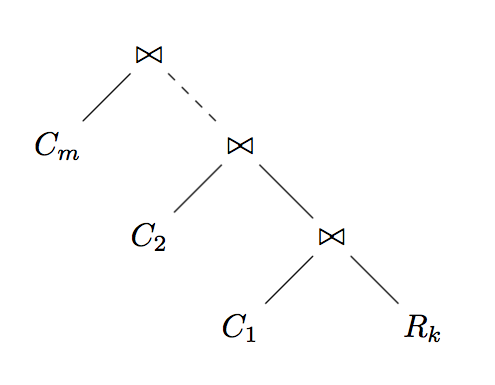
\includegraphics[scale=0.4]{03_Regeln/00_media/ReducedQueryTree.png}
  \caption{Reduzierter Query-Tree}
  \label{ReducedQueryTree}
\end{figure}



$Beweis:$ Das Ziel des Lemma ist es zu zeigen, dass aus einem gegebenen kreuzproduktfreien Baum die Relation mit der höchsten Nummer ($R_k$) so nach oben verschoben werden kann, dass diese Relation zuletzt gejoint wird.

Sei $R_k$ die Relation mit der höchsten nummer und die Relationen $R_1, ..., R_{k-1}$ andere Relationen innerhalb des Baums. Unter verwendung der Kummutativitätsregel können wir den gegebenen Query-Tree so transformieren, dass ein Baum entsteht, wie er in Abbildung \ref{ReducedQueryTree} zu sehen ist. $C_1, C_2, .. C_m$ sind hierbei Join Trees, die wiederum aus einer Menge von Relationen bestehen. Da die Anwendung von Kommutatvitität niemals ein Kreuzprodukt erzeugt, ist diese und alle zwischen Zustände des Graphen kreuzproduktfrei. Die in $m$ angegebene Zahl ist nicht nur die höchste Nummer mit der ein $C$ bezeichnet wird, sondern drückt zudem die Tiefe von $R_k$ aus.

\textbf{Basis Fall:} Bei einer Tiefe von $m = 1$, ist die Relation $R_k$ automatisch die letzte Relation die gejoint wird. Daher ist das Lemma für diesen Fall korrekt.

\textbf{Induktion:} Angenommen Lemma 1 ist korrekt für $m <= j$. Sei die Tiefe von $R_k$ $m = j+1$. 

\begin{figure}[ht]
  \centering
  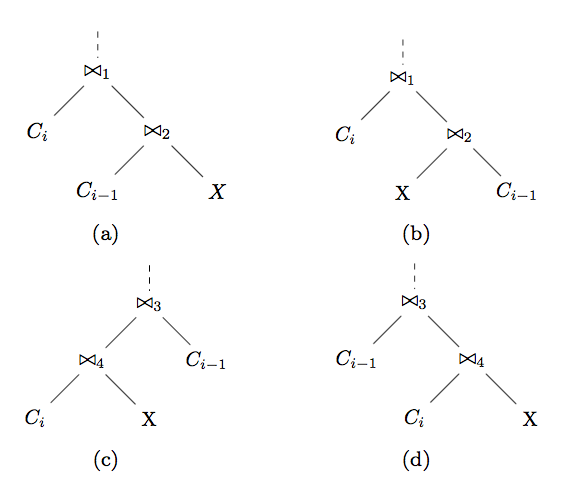
\includegraphics[scale=0.4]{03_Regeln/00_media/SwapC1.png}
  \caption{Tausch von $C_i$ und $C_{i-1}$}
  \label{SwapC1}
\end{figure}



Angenommen Lemma 1 sei korrekt für $ m <= j$ und die Tiefe von $R_k$ $m = j + 1$. Angenommen es existiert ein Subbaum aus $R_1, R_2,.. , R_k$. Solange $R_k$ die letzte Relation ist die gejoint wird, dann gibt es ein $C_1$ das jeoint werden kann mit mindestenens einem andereren der $C$ beispielsweie mit $C_i$. Dadurch ist es möglich, dass $C_i$ nach unten zu $C_1$ verschoben wird indem die folgende Sequenz an Regeln angewendet wird.

Wie in Abbildung \ref{SwapC1} a zu sehen ist, gibt es ein X, das die rechte Seite eines Subtrees darstellt und der mit $C_{i-1}$ gejoint ist. Wir wenden auf den Join $\Join_2$ die Kommutativitätsregel an, so entsteht Abbildung \ref{SwapC1} b. Auf den Join $\Join_1$ wird linke-Assoziativität angewendet, so entsteht $\Join_3$. Mit einer finalen Anwendung von Kommutativität auf $\Join_3$ entsteht \ref{SwapC1} d.

Jeder Zwischenschritt ist kreuzproduktfrei, da $C_i$ ein Join Prädikat mit $C_1$ besitzt welches Teil des Subtrees $X$  wie auch $C_{i-1}$.

Am Ende der Sequenz von Transformationen ist $C_i$ einen Schritt näher an $C_1$ gerückt. Jedes Mal, wenn die Sequenz angewendet wird, rückt $C_1$ noch ein Stück näher.

Zum Schnluss ist $C_1$ auf dem selben Level wie $C_i$ wie es in Abbildung \ref{} a zu sehen ist.  Mit Hilfe von linker Assoziativität kann dann der Baum aus Abbildung \ref{} b erzeugt werden.  Dieser Baum ist auch kreuzproduktfrei, da $C_i$ und $C_1$ ein gemeinsames Prädikat besitzen und so tuen es auch $R_k$ und $C_1$.

Die Tiefe von $R_k$ ist nun von $j + 1$ auf $j$ verkleinert, dies induziert, dass die Hypothese für $m <= j$ korrekt ist und somit das Lemma bewiesen.


\begin{lem}
Gegeben Sei ein Join-Graph $G$ und ein kreuzproduktfreier Query Tree, der aus G gebildet wurde, dann kann dieser in einen links-tiefen Tree basierend auf $G$ transformiert werden mit Hilfe von $RS-B1-CPS$.


\end{lem}

$Beweis:$ Angenommen die Relationen eines links-liefen Join-Trees sind nummeriert von $R_1$ bis $R_n$. Wie bereits zeigt in Lemma 1, ist die Transformation mit RS-B1-CPS möglich, die $R_n$ nach oben bewegt, sodass sie die letzte Relation ist, die gejoint wird. Die Regeln, die in RS-B1-CPS sind können angewendet werden, um den linken subTree des Resukatsbaums in einen Baum mit $R_{n-1}$ nach oben zu schieben. Es ist einfach zu zeigen, dass mit Hilfe von Indution, dass der gewünschte link-tiefe Baum erzeugt werden kann durch die Anwendung von RS-B1-CPS.

\begin{lem}
Gegeben sei ein Join Graph G. Ein beliebiger link-liefer Join Tree $T1$ kann in jeden kreuzproduktfrein Query Tree T2 transformiert werden mit RS-B1-CPS.
\end{lem}

$Beweis:$ Wie in Lemma 2 zu sehen, kann jeder Kreuzproduzktfreie Join Treee T2 in einen kreuzproduktfreien links-liefen Baum transfomriert werden. Wenn diese Sequenz, die zur Erzeugung des links-liefen baums ausgeführt wird, rückwärts abläuft, kann so der links-liefe Baum aus dem beliebigen Baum gebildet werden. Wobei anstatt von linker-Assoziativität rechte-Assoziativität zum Einsatz kommen muss. Zwar ist rechte-Assoziativität Teil nicht Teil von RS-B1-CPS kann jedoch mit Hilfe von Assoziativität und Kommutativität hergestellt werden. 
 

\begin{teo}
Die Regelmenge RS-B1-CPS ist vollständig, gegeben sei ein beliebiger kreuzproduktfreier Join Tree T1. dann ist es möglich alle anderen kreuzproduktfreien Bäume aus diesem zu erstellen, indem eine Reihe von Regeln als RS-B1-CPS angewendet werden.
\end{teo}

$Beweis:$ Der Bereis für die Vollständigkeit lässt sich aus Lemma 2 und Lemma 3 ableiten. Wir können jeden Tree in einen links-tiefen Baum umwnadeln und dies wieder 




Es wurde angenommen, dass für einen kreuzproduktfreien Baum mit den Relationen $R_1, R_2, ..., R_k$


\subsection{Unvollständigkeit von RS-B2}

\begin{figure}[ht]
  \centering
  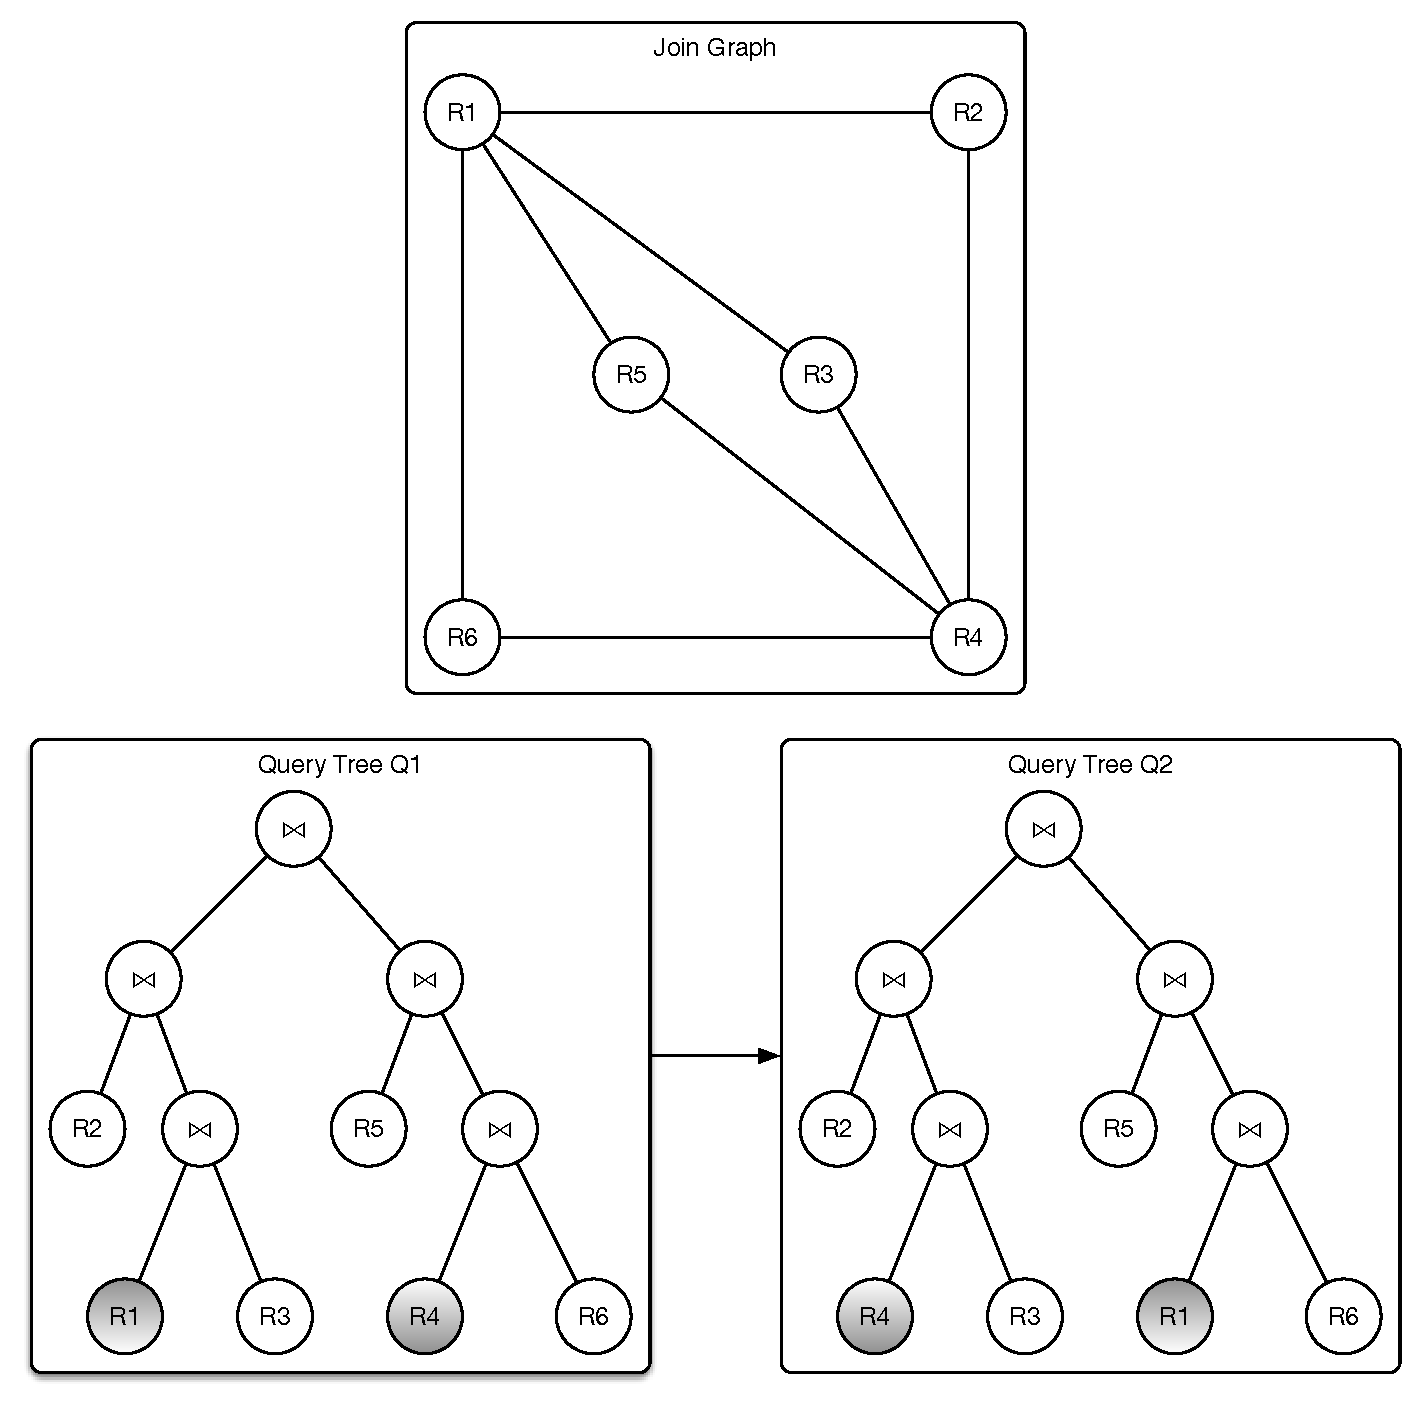
\includegraphics[width=\textwidth]{02_Related_Work/Graphs.pdf}
  \caption{Incompletness of RS-B2-CPS}
  \label{Incompleteness_RS-B2-CPS}
\end{figure}


Die Unvollständigkeit wurde mit Hilfe eines Beispiels belegt. Als Beispiel wurde der Bushy-Tree gewählt, der in Abbildung \ref{Incompleteness_RS-B2-CPS} zu sehen ist. Mit Hilfe der Regeln aus der Regelmenge RS-B2 sollte der initale Plan () in den Plan () umgewandelt werden. Dabei werden die vier Regeln der Regelmenge angewendet.

\begin{itemize}
\item Mit der Kommutativitätsregel ist es möglich ein Spiegelbild des original Baums herzustellen, aber nicht den Plan grundlegend zu verändern.
\item Bei der Anwendung von linker Assoziativität auf den Root-Knoten des Baum würde ein neuer Baum erzeugt werden dessen
\item Das Ergebnis von rechter Assoziativität ist symmetrisch zu linker Assoziativität.
\end{itemize}


Welche Regel auch immer auf den Baum angewendet wird, es ist nicht möglich den einen in den anderen Baum zu transformieren.

\subsection{Unvollständigkeit von RS-B2 mit Hilfe von PyroJ}

Mit Hilfe des Optimierers PyroJ - sein Aufbau wird in \ref{sec:pyroJ} behandelt - wurden die Regelsets ebenfalls auf ihre Vollständigkeit hin geprüft. Es wurde angenommen, dass zwei Ergebnismengen dann gleich sind, wenn die Anzahl der Äquivalenzklassen und die Anzahl der Operatorknoten gleich ist. Da wie zuvor festgestellt RS-B1 vollständig ist, wurde RS-B1 als Benchmark für andere Regelsets genutzt. Als Test-Case wurden Starqueries verwendet. Wie in Tabelle \ref{} zu sehen ist, wurde mit Hilfe von RS-B2 erheblich weniger Operatoren-Knoten erzeugt als mit RS-B1. \cite{} schlisst daher darauf, dass RS-B2 unvollständig ist.

Ebenfalls stellt \cite{} hervor, dass eine bestimmte Anfrage (Anfrage 7 des TPC-DS Benchmarks) bei der Nutzung des RS-B2 eine um 1.86 höher geschätzte Kosten als RS-B1 verursacht hatte.



\subsection{Hinweise auf Unvollständigkeit}
\section{GraphRule und Unvollständigkeit von RS-B2}

Die von Pellenkoft et al. entwickelten Regelsets, dienen als Grundlage für regelbasierte Optimierer wie Volcano. \cite{shanbhag2014optimizing} untersuchten die Vollständigkeit der vorgestellten Regel und fügten den bestehenden Regelsets ein neues hinzu, das alle andere Regelsets zum Join Reordering obsolet macht und zudem eine erheblich bessere Performance liefert.

Die Untersuchungen \cite{shanbhag2014optimizing} wurden mit dem Optimierer PyroJ durchgeführt. PyroJ ist ein Optimierer, der basierend auf Pyro \cite{roy2001multi} erstellt wurde und dem Volcano Optimizer nachempfunden ist. Zuerst wurden die Regelsets auf ihre Vollständigkeit hin geprüft. Neben der Prüfung auf Vollständigkeit konnte auch die neue Regel GraphRule implementiert und so bzgl. ihrer Performance getestet werden.



\subsection{Implementierung von PyroJ}

PyroJ basiert auf dem von \cite{roy2001multi} in C++ Implementierten Optimierer Pyro und wurde automatisch von C++ nach Java übersetzt. Der Optimierer Pyro wurde nach dem Vorbild des Volcano Optimierers entwickelt. Volcano wurde als Vorbild gewählt, da es sich bei Volcano um einen hoch-respektierten, state-of-the-art, regelbasierten Optimierer handelt, der auch die Basis von kommerziellen Datenbanksytemen wie MS SQL Server ist. Außerdem ist Volcano, wie zuvor besprochen, hoch erweiterbar: Das Datenmodell, Executionmodell ist leicht erweiterbar, Transformationsregeln und Operatoren lassen sich hinzufügen. 

Einer der Unterschiede zwischen Volcano und Pyro ist die Trennung zwischen logical / physical Plan Generierung und der Suche nach dem optimalen Plan. Im Gegensatz zu Volcano werden erst alle logische Pläne für einen \ac{LQDAG} generiert, daraufhin werden alle Pläne in physische Pläne umgesetzt und basierend auf diesen Plänen der günstigste Plan ausgewählt.

Der Volcano Optimizer hingegen berechnet zuerst einen logischen Plan und generiert für diesen Plan dann alle physischen Pläne. Für diese Pläne wird der günstigste Plan gesucht. Die anderen Pläne müssen nicht mehr im Speicher vorgehalten werden. Daraufhin kann dann der nächste logische Plan generiert werden und die Kosten des günstigsten Plans mit dem bisher günstigsten Plan verglichen werden. Der Vorteil dieses Verfahrens ist, dass gerade bei großen Search Spaces der Plan im Speicher gehalten werden kann und suboptimale Pläne nicht länger als nötig gespeichert werden.

Genau wie das Volcano Projekt wird eine Memofunktion verwendet. \cite{roy2001multi} weist daraufhin, dass diese Memofunktion erst später dem Volcano Optimizer hinzugefügt wurde. Dadurch war es beispielsweise möglich, dass bei einer Anfrage, die aus $(A \Join B \Join C) \cup (B \Join C \Join D)$ zwei Äquivalenzknoten für den Knoten $B \Join C$ gebildet werden, obwohl alle Teilpläne von $A \Join B$ immer äquivalent sein werden und somit kein Grund besteht, die Pläne mehrfach zu berechnen. Pyro verwendet eine Memodatenstruktur, um die mehrfache Generierung des selben Teilplans zu unterbinden.

Ein weiterer Unterschied zu Volcano ist, dass es  bei Pyro kein Optimizer generiert wird, sondern der Optimizer von vornherein in C++ geschrieben ist. Eine Übersetzung aus einem Description\-File hin zu C\-Code findet daher nicht statt.

\subsection{Getestete Regeln und Regelsets}

\cite{shanbhag2014optimizing} und \cite{roy2001multi} geben an, dass sie die Regelsets \textit{RS-B0}, \textit{RS-B1} und \textit{RS-B2} implementieren. Im Gegensatz zu Pellenkoft wird im Regelset \textit{RS-B1} nicht die Regel Swap verwendet, sondern Left\-Associtativity (vgl. \ref{PellenkoftVsPyro}). Beide Regeln sind jedoch semantisch ähnlich genug und können mit Hilfe von Kommutativität in einander überführt werden. Ebenfalls ist eine genaue Unterscheidung der Reihenfolge der Anwendung, ähnlich wie bei Volcano nicht möglich. Alle Regeln laufen immer in einer vorgegeben Reihenfolge ab.

\begin{table}[ht]
\begin{tabular}{|l|l|l|}
\cline{1-3}
{\bf Regelmenge} & {\bf Pellenkoft}                                                                                                  & {\bf Pyro(J)}                                                                                                       \\ \cline{1-3}
{\bf RS-B0}   & \begin{tabular}[c]{@{}l@{}}Left Associativity\\ Right Associativity\\ Commutativity\end{tabular}            & \begin{tabular}[c]{@{}l@{}}Left Associativity\\ Right Associativity\\ Commutativity\end{tabular}              \\ \cline{1-3}
{\bf RS-B1 }  & \begin{tabular}[c]{@{}l@{}}Swap\\ Bottom Commutativity\end{tabular}                                         & \begin{tabular}[c]{@{}l@{}}Left Associativity\\ Commutativity\end{tabular}                                    \\ \cline{1-3}
{\bf RS-B2 }  & \begin{tabular}[c]{@{}l@{}}Left Associativity\\ Right Associativity\\ Commutativity\\ Exchange\end{tabular} & \begin{tabular}[c]{@{}l@{}}Left Associativity\\ Right Associativity\\ Commutativity\\ Exchange\end{tabular}   \\ \cline{1-3}
\end{tabular}
\caption{Unterschiede zwischen Pellenkoft und Pyro(J)}
\label{PellenkoftVsPyro}
\end{table}




\subsection{Unvollständigkeit von \textit{RS-B2}}



\begin{figure}[ht]
  \centering
  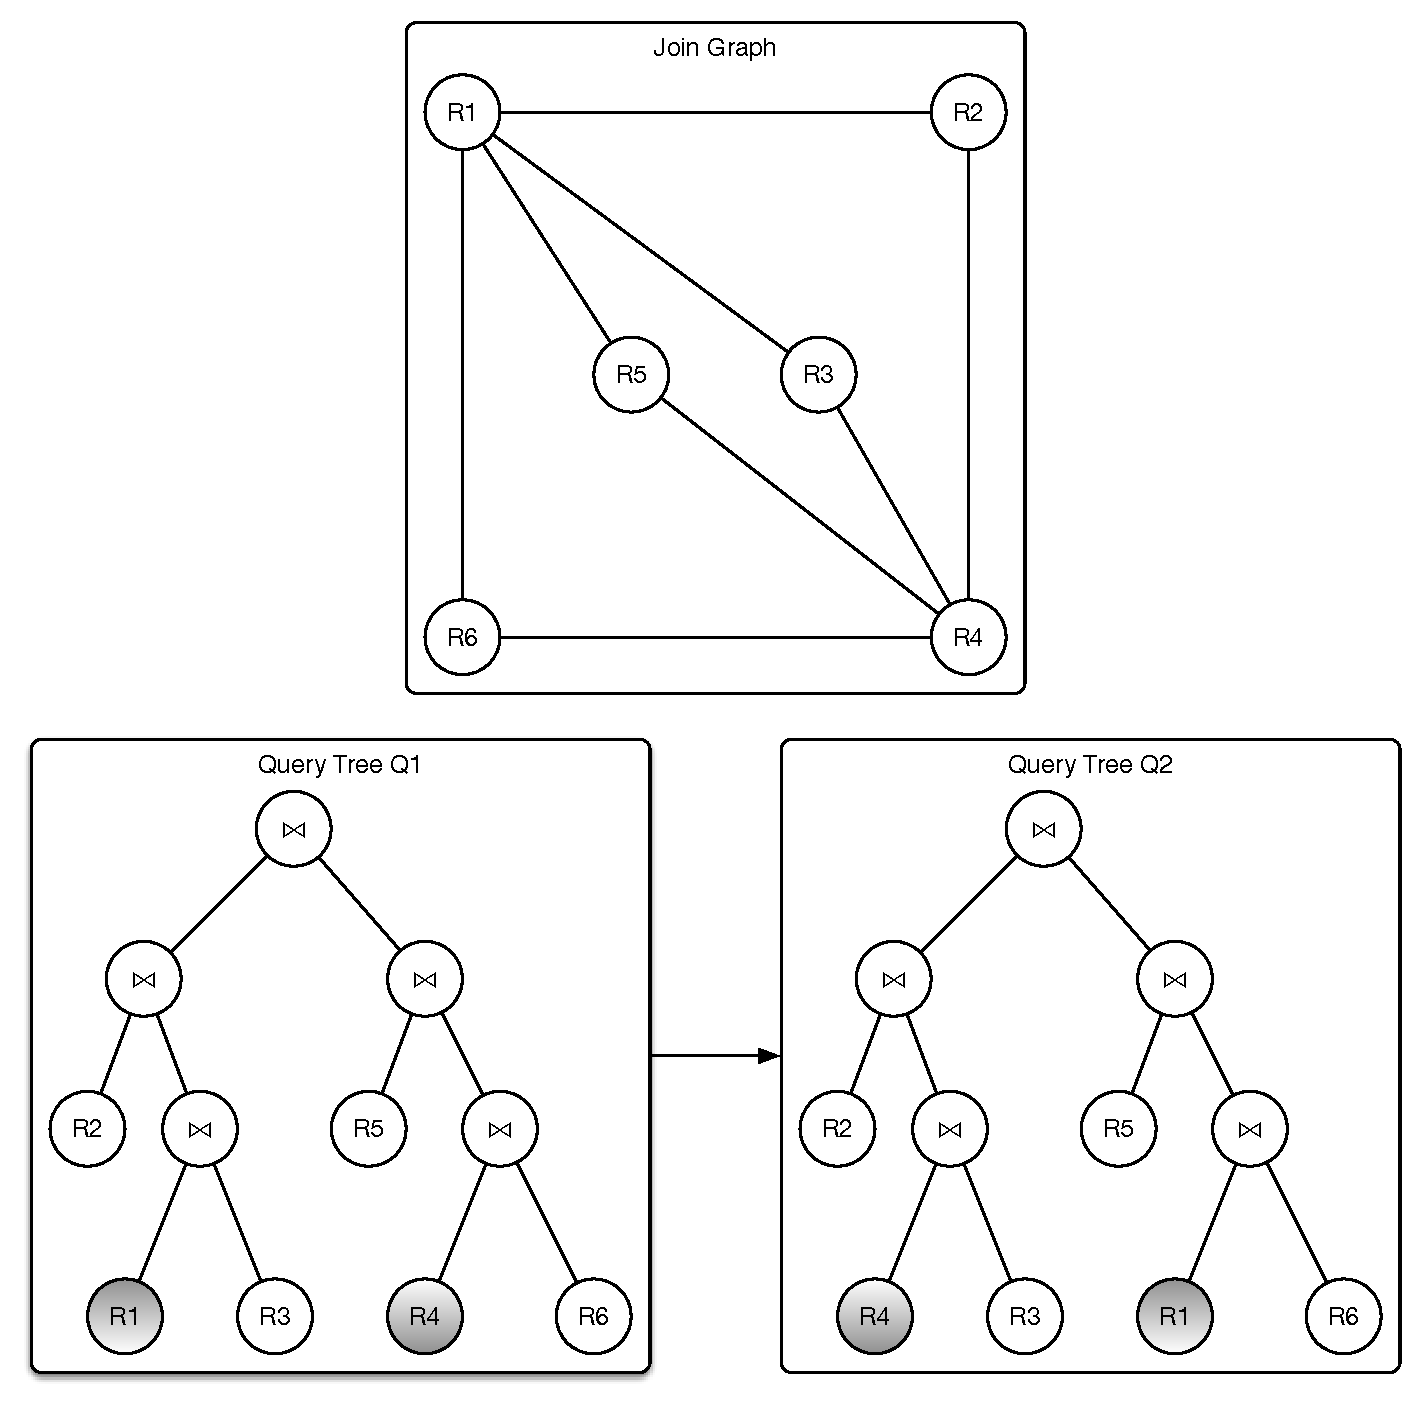
\includegraphics[width=\textwidth]{02_Related_Work/Graphs.pdf}
  \caption{Incompletness of RS-B2-CPS}
  \label{Incompleteness_RS-B2-CPS}
\end{figure}


Die Unvollständigkeit von \textit{RS-B2} wurde auf zwei Arten gezeigt. Auf der einen Seite wurde an Hand des Beispiel \ref{Incompleteness_RS} gezeigt. Im konkreten Beispiel sollte \textit{R1} und \textit{R4} getauscht werden, wobei das Regelset \textit{RS-B2} zum Einsatz kommen sollte. Anhand des gegebenen Join Graphen ist die Transformation zwar Teil des Suchraums, kann jedoch durch die Regeln nicht erreicht werden. Das Regelset ist daher unvollständig.

Ebenfalls wurden unterschiedliche Abfragen mit Hilfe des Optimierers optimiert und dahingehend geprüft, ob die selbe Menge an Plänen aus den unterschiedlichen Regelsets entstehen kann. Wie erwartent war die Menge der Pläne, die aus \textit{RS-B0} nur \textit{RS-B1} entstanden sind gleich, die Menge der \textit{RS-B2} Pläne stark reduziert. (vgl. \ref{tabelle)}.

Da nicht alle Pläne gefunden werden konnten, liegt es nahe, dass der optimale Plan möglicherweise nicht Teil des erforschten Suchraums ist. \cite{shanbhag2014optimizing} stellen fest, dass das Ergebnis mit \textit{RS-B2} erzeugt wurde bzgl. der berechneten Kosten um den Faktor 1.86 schlechter war, als die Pläne, die mit Hilfe eines vollständigen Regelsets erzeugt wurden. Wie genau die Zahl 1.86 zustande gekommen ist, ist nicht genauer begründet.

Es lässt sich also feststellen, dass mit Hilfe des Regelsets \textit{RS-B2} weniger Pläne im Suchraum gefunden werden konnten, als mit Hilfe des Regelsets \textit{RS-B1} bzw. \textit{RS-B2}. Außerdem wurde festgestellt, dass Pläne aus unvollständigen Regelsets nicht immer den optimalen Plan beinhalten.





\subsection{Unvollständigkeit von RS\-02}




\cite{shanbhag2014optimizing} stellt fest, dass RS-B0-CPS und RS-B1-CPS vollständig sind. Die Vollständigkeit von RS-B2-CPS wird jedoch in Frage gestellt und die Unvollständigkeit mit Hilfe eines Beispiels belegt. Als Beispiel dient eine Menge von Relationen, die mit Hilfe des Jointrees J (\ref{fig:Incompleteness_RS-B2-CPS}) miteinander gejoint sind. Der Initale Anfragebaum \textit{Q1} ist in \ref{fig:Incompleteness_RS-B2-CPS} dargestellt. Das gewünschte Ergebnis nach einer Transformation \textit{Q2}  findet sich in \ref{fig:Incompleteness_RS-B2-CPS}. 

Bei \textit{RS-B2-CPS} dürfen die Regeln \textit{R2}, \textit{R3}, \textit{R4} nur jeweils einmal auf einen Join-Operator angewendet werden. Keine der Regeln darf danach auf den neu generierten Operator angewendet werden. Die In \ref{fig:Q1} und \ref{fig:Q2} zeichnet sich dadurch aus, dass die Relationen \textit{R1} und \textit{R4} vertauscht sind.


Die Vollständigkeit wurde auch mit Hilfe des PyroJ Optimierers geprüft. Hierbei wurde an Hand von Star-Queries  die Unvollständigkeit belegt. Wie in Abb. \ref{CompletenessResults} zu sehen, wurden mit Hilfe von \textit{RS-B2} nur knapp die Hälfte aller äquivalenten Pläne gefunden. Ebenfalls wird betont, dass die geschätzten Kosten des besten Plans, der durch \textit{RS-B2} erzeugt wurde um den Faktor 1.86 im Vergleich zu \textit{RS-B1} niedrigere geschätzte Kosten hatte.







\subsection{Vorschlag von RS-Graph}

\subsection{JOIN SETS}

Basierend auf dem bisherigen Wissen, wurden durch X und Y einige neue Begriffe festgelegt: W.
Ein Base Equivalenz Knoten in einem expandierten LQDAG ist ein Äquivalenzknoten, der keinen Join Operator als Kinder hat. Ein solcher Knoten kann entweder eine Relation sein oder darf keine Join Operatoren als Kinder beinhalten.

Ein Join Tree ist in einem expandierten LQDAG ein Baum in der LQDAG dessen Wurzel ein Äuqivalenzknoten und jeder interne Knoten entweder ein Äquivalenzknoten oder ein Join Operator und jeder untergeordneter Knoten ein Äuqivalenzknoten ist.

Der Maximale JOIN Tree ist in einem expandierten LQDAG ein Join Tree, bei dem jeder Leaf Knoten ein Base Equivalence Node ist.

Ein Join-Set für einen Äquivalenzknoten E ist in einem expandierten LQDAG ein Paar $J = (S, P)$ bei dem S ein Set von Äquivalenzknoten ist, deren 

\subsection{Regelmenge RS-Graph}
Neben den bereits etablierten Regeln wird eine neue Regel für den Volcano Optimizer von \cite{shanbhag2014optimizing} vorgestellt. Die neue Transformationsregel \emph{RS-Graph} ersetzt die bisherigen Regeln und die bisherigen Regelsets. Die neue Regel erzeugt basierend auf einem Planknoten direkt alle möglichen äquivalenten Pläne. Somit sind alle Pläne unter einem bestimmten Äquivalenzknoten mit der Anwendung nur einer Regel erzeugt.

Die Regel \emph{RS-Graph} verwendet dazu die Subroutine $GraphRule$. Sie wird auf den Join Tree angewendet, falls die beiden mit einem Operator verbundenen Knoten A und B und deren Mitterknoten $P$. Für jedes Paar der J %\emph{equivalence nodes A,B and parent equivalence node P. For each pair of join-set (jsA,jsB) ∈ A.JoinSets∗B.JoinSets, we merge the pair to form a join-set js. We define the merge of the two join-sets jsA = (V1,P1) and jsB = (V2,P2) as (V1∪V2,P1 ∧P2).}

Um wiederholte Berechnungen des selben Join Trees zu vermeiden wird zudem geprüft, ob der Eltern-Äquivalenzknoten bereits $js$ beinhaltet. $$To check if two join- sets at an equivalence node are equal, it is sufficient to check if they have same equivalence nodes. If the join-sets have the same equivalence nodes, then they will also have the same predicates.$$

Für alle Join Sets $js$ des Parent nodes werden daraufhin zuerst alle JOIN partitionen gebildet bei denen $S_1 \Join S_2$ mit 

Sollte der $js$ noch nicht existieren, wird dieser dem JOIN Set hinzugefügt. Ein Graph wird basierend auf den $js$ gebildet, der mit Hilfe der Methode Partition in alle Partitionen getrennt wird. Aus denen werden wiederum Bäume erstellt, die an das Resultat zurückgegeben werden.

Die SubRoutine Create Graph, gibt ein JOIN Set, das JS einen Join Graphen aus, der




\subsection{Diskussion}
Die Implementierung der neuen Regel wurde in einem Java basierten regelbasierten Op den Äquivalenzklassen neue Felder hinzugefügt werden.

Die Generierung der Resultate findet ohne Pruning statt und Kosten für die Kostenberechnung werden nicht einbezogen. Ebenfalls bleiben Regeln bestehen, die für denn SELECT Pushdown verantwortlich sind, als Teil der Normalisierungsphase. 

Es wurden sowohl Star, Chain als auch Clique Queries getestet. Die Experimente fanden auf einem Intel i5 3.5 GHz mit 8 GB Ram statt. Es wurde festgestellt, dass die Geschwindigkeit der Optimierung verbessert werden konnte, dadurch, dass die Optimierung mehrfach durchgeführt wurde. Dieses Verhalten wurde auf Javas JIT Kompilierungsstrategie zurückgeführt, die erst den Code kompiliert, wenn er auch tatsächlich gebraucht wird. Um sicherzustellen, dass der Kompilierte Code nicht wieder während der Ausführung vergessen wird, mussten spezielle Flags für die JVM gesetzt werden. Das Ergebnis war, dass die Dauer zwar verglichen zu den schnellsten Tests ohne das Flag langsamer, aber dafür konstant blieb.

Ebenfalls wurde bei Regelmenge $RS_B1$ geprüft, ob der gesamte Search Space erreicht wurde, indem die Anzahl der Äquivalenten Knoten und Operatoren im LQDAG gezählt wurden. Diese Zahl wurde mit der Zahl der Knoten in RS-Graph verglichen. Da beide Zahlen gleich waren, wird davon ausgegangen, dass beide Regelsets das selbe Ergebnis erzeugen. Eine Prüfung, die dies belegt fand aus technischen Gründen nicht statt.






Ersetzten X und Y die bisher gezeigten Regeln des Volcano Optimierers mit einer neuen Transformationsregel: RS-Graph. Die Regel kommt zur Anwendung, falls ein Graph dem Pattern $E_1 \Join E_2$ entspricht. Ist dies der Fall wird die Funktion $GraphRule(\Join, E_1, E_2, parent)$ aufgerufen. Sie erzeugt ein Set von allen Join Operatoren unter dem Äquivalenzklasse des $parent$-Knotens.







\subsection{Partition zu Graph}



Die Methode Partition gibt eine Menge von Partitionen zurück. Jede Partition bezeichnet eine Menge von Knoten. Sowohl $S_1$ als auch $G\\S_1$ sind Teil dieser Menge, falls beide zwischen beiden im Join-Graphen miteinander verbunden sind. Im Gegensatz zu anderen Regeln, die pro Anwendung der Regel nur immer einen neuen Knoten zurückgegeben haben, gibt die neue Regel immer Bäume zurück, die alle möglichen Join Operatoren unterhalb des ROOT Operators beinhalten.





Das bestehende Regel-Framework von Volcano wurde von \cite{shanbhag2014optimizing} mit einem neuen Regelset und einer neuen Regel erweitert. Das neue Regelset Graph Rule soll alle bestehenden Regeln zur JOIN-Tree Enumeration ersetzen. Im Gegensatz zu den vergleichsweise ineffektiven Regelsets, die bisher bekannt waren, setzt die neue Regel auf state-of-the-art, kreuzproduktfreie Join-Enumeratoren zur Suche nach äquivalenten Plänen. Damit kombiniert die neue Regel die Vorteile eines hoch erweiterbaren Systems wie Volcano mit der Geschwindigkeit von neuartigen Join-Enumeratoren.

Die neue Regel gibt nicht nur eine neue Variante des Query-Trees zurück, sondern bestimmt gleich auf einmal alle äquivalenten Pläne. Die Erweiterbarkeit des Volcano-Optimierers ermöglicht es auch eine solche komplexe, neue Regel zu implementieren.

Die neue Regel wird in drei Schritten umgesetzt. Zuerst werden die Subtrees bestimmt, auf die ein Paritionierungsalgorithmus im nächsten Schritt angewendet werden kann. Mit Hilfe der einzelnen Partitionen werden dann neue Bäume aufgebaut, die als alternative Pläne zurückgegeben werden. Diese drei Schritte sind auch in Abb. \ref{GraphRule} zu sehen.

\subsection{Routinen}





Um die Funktion der neuen Regel im Detail zu beschreiben, führt \cite{shanbhag2014optimizing} eine Reihe neuer Begriffe für einen Baum ein:

\begin{itemize}
\item \textit{Base Equivalence Node}: dieser Knoten bezeichnet einen Äuqivalenzknoten, der keine JOIN-Operatoren als dessen Kinder besitzt.
\item \textit{Join Equivalence Node}: dieser Begriff bezeichnet einen Äquivalenzknoten, der mindestens eine JOIN Operation untergeordnet hat.
\item \textit{Maximal Join Tree}: Dieser Baum ist ein Baum, der entweder Äquivalenzknoten oder einen JOIN Operator untergeordnet hat.
\item Ein \textit{Maximal join Tree} ist ein Baum, dessen Kinder immer EuqivalenceNodes sind.
\item Ein \textit{Join Set} für einen Äquivalenzknoten E ist ein Paar $J = (V, P)$ bei dem $V$ ein Set von Äquivalenknoten ist und deren Kinder seine 
\end{itemize}


\subsection{Implementierung}
Die Implementierung des neuen Regelsets wurde auf Basis des Query Optimierers PyroJ vorgenommen. PyroJ ist eine Übersetzung des in C++ entwickelten Optimierers Pyro, der an der Universität Bombay entwickelt wurde und das Volcano-Framework implementiert.

Alle Tests wurden auf einem Computer mit Intels Core i5 3.5 GHz mit 8 Gbyte Arbeitsspeicher und Ubuntu 11.10 durchgeführt. Die genaue Java Version und Einstellungen der JVM sind (fast) vollständig unbekannt.

Wie von \cite{shanbhag2014optimizing} beschrieben, wurde während er Performance Test festgestellt,dass sich die Dauer für die Ausführung einer Optimierung stark unterscheidet.Für die Durchführung einer Optimierung wurden zu Beginn erheblich höhere Werte festgestellt. Gerade die ersten Anfragen hatten eine besonders hohe Laufzeit. Erklärt wurde dieses Verhalten durch den Java \ac{JIT}-Compiler. Ebenfalls wurde erkannt, dass der Java eigene Code Optimierer HotSpot die Ergebnisse verfälschen kann. 

Während der Performance Tests wurde festgestellt, dass sich.........


\subsection{Probleme auf Grund der Plattformwahl}
Die Implementierung der neuen Regel wurde auf Basis von PyroJ vorgenommen. PyroJ ist eine Übersetzung des von ITT Bombay entwickelten Systems Pyro, das eine Implementierung des Volcano-Frameworks ist. PyroJ, das in Java implementiert ist, entstand durch eine automatische Konvertierung des C++ Codes von Pyro. 

Die Implementierung der Experimente wurde auf Basis von PyroJ vorgenommen. PyroJ ist eine Übersetzung des in C++ geschriebenen Query Optimierers Pyro nach Java. Der Optimierer wurde an der IIT Bombay gebaut und ist eine Implementierung des Volcano Optimization Frameworks.

Die Experimente wurden auf einem Intel Core i5 3.5 GHz Computer mit 8 Gbyte Arbeitsspeicher und Ubuntu 11.10 vorgenommen. Es wurde festegestellt, dass die Implementierung des Codes in Java verglichen zu C++ einigen Overhead generiert, der die Laufzeit der Optimierung negativ beeinflusst. Ebenfalls wurde festgestellt, dass die Laufzeit zur Optimierung einer Anfrage erheblichen Schwankungen unterlegen ist. Insbesondere konnten stark unterschiedliche Laufzeiten bei den selben Queries festgestellt werden. Queries, die zu Beginn ausgeführt wurden, wurden langsamer ausgeführt. Dieses Phänomen wurde auf den Java JIT-Compiler (HotSpot) zurückgeführt. Dieser kompiliert nur die zur Ausführung notwendigen Teile des Programms und führt Optimierungen zur Laufzeit durch. Um konstante Laufzeiten für die selbe Anfrage zu erzielen, wurde nach eigenen Angaben die JIT-Kompilierung ausgeschaltet. Außerdem wurde das Java HotSpot JVM flag $-XX:CompileThreshold=1$ gesetzt und einige große Queries ein paar mal optimiert, um sicherzustellen, dass alle Funktionen auch kompiliert werden bevor sie ausgeführt werden.
 

\subsection{Kritik} \todo{Wo soll dieser Teil eigentlich hin? Evaulation/ Related Work / Implementierung}


Die Implementierung des Frameworks wirft einige Fragen auf. Auf der einen Seite wird durch den Autor selbst festgestellt, dass durch die Wahl einer anderen Code Basis (C++ statt Java) Ergebnisse mit weniger Overhead erzielt werden könnten. Warum also die Entscheidung zur Implementierung in Java gefallen ist, bleibt unbeantwortet.

Auch die Probleme, die durch den JIT Compiler entstanden sind, sind außergewöhnlich. Zuerst wurde die Kompilierung nach eigenen Angaben abgeschaltet und dann wiederum sichergestellt, dass alles kompiliert wurde, indem große Anfragen optimiert wurden. Was genau mit dieser Aussage gemeint ist bleibt unbeantwortet.  Ich nehme an, dass nur das JVM Flag $-XX:CompileThreshold=1$ gesetzt wurde. Dieses Flag gibt an, nach wie vielen Methodenaufrufen ein Stück Java Code in Maschinencode kompiliert wird. Der Standardwert liegt bei 10000 \cite{oracle2015VMOptions}. Dank dieses Flags wird bereits beim ersten Aufruf einer Methode die Methode auch kompiliert. Warum dieser Umweg gewählt wurde, bleibt wage.

Ein weiterer Grund für Fehler bei der Messung kann die Wahl der Plattform im Allgemeinen sein. Da die Ausführung des Programms zu jedem beliebigen Zeitpunkt durch die Garbage Collection unterbrochen werden kann, können Messungen der Laufzeit nur schwer vorgenommen werden. Um wenigstens einen Hinweis auf diese Messfehler zu finden, wäre eine Nutzung der JVM Flags $ -verbose:gc -XX:+PrintGCDateStamps -XX:+PrintGCDetails$ möglich gewesen. Diese Flags geben an, wann die Garbage Collection zuschlägt und wieviel Zeit diese zur Ausführung benötgt. \cite{andreasson2015JVM}  


Warum also trotz all dieser möglichen Fehlerquellen und Ungenauigkeiten gerade Java zum Einsatz gekommen ist, ist unklar und wenig verständlich. Insbesondere da eine Alternative in C++ mit Pyro bereitstand.





\section{Performance von RS-Graph zu anderen Regelmengen}


Ähnlich wie \cite{} wurde auch hier die Performance der einzelnen Regelmengen gemessen. Im Gegensatz zu den vorherigen Messungen - sie wurden in Kapitel 3 beschrieben, wurde die Kostenbrechnung mit einbezogen. Genau wie bei den Test in Kapitel 3 wurden die unterschiedliche Formen einbezogen und unterschiedliche Anzahlen an Relationen verwendet. Im Gegensatz zu \cite{} werden jedoch nur die Regelmengen getestet, die auch kreuzproduktfrei sind. 

Die Auswertung beginnt mit den Kettenförmigen Graphen. Die Anzahl der Relationen wurde immer weiter gesteigert. 


%\section{GraphRule und Unvollständigkeit von RS-B2}

Die von Pellenkoft et al. entwickelten Regelsets, dienen als Grundlage für regelbasierte Optimierer wie Volcano. \cite{shanbhag2014optimizing} untersuchten die Vollständigkeit der vorgestellten Regel und fügten den bestehenden Regelsets etwas Neues hinzu, das alle andere Regelsets zum Join Reordering obsolet macht und zudem eine erheblich bessere Performance liefert.

Die Untersuchungen \cite{shanbhag2014optimizing} wurden mit dem Optimierer PyroJ durchgeführt. PyroJ ist ein Optimierer, der basierend auf Pyro \cite{roy2001multi} erstellt wurde und dem Volcano Optimizer nachempfunden ist. Zuerst wurden die Regelsets auf ihre Vollständigkeit hin geprüft. Neben der Prüfung auf Vollständigkeit, konnte auch die neue Regel GraphRule implementiert und so bzgl. ihrer Performance getestet werden.



\subsection{Getestete Regeln und Regelsets}

\cite{shanbhag2014optimizing} und \cite{roy2001multi} geben an, dass sie die Regelsets \textit{RS-B0}, \textit{RS-B1} und \textit{RS-B2} implementieren. Im Gegensatz zu Pellenkoft wird im Regelset \textit{RS-B1} nicht die Regel Swap verwendet, sondern Left\-Associtativity (vgl. \ref{PellenkoftVsPyro}). Beide Regeln sind jedoch semantisch ähnlich genug und können mit Hilfe von Kommutativität in einander überführt werden. Ebenfalls ist eine genaue Unterscheidung der Reihenfolge der Anwendung, ähnlich wie bei Volcano nicht möglich. Alle Regeln laufen immer in einer vorgegeben Reihenfolge ab.

\begin{table}[ht]
\begin{tabular}{|l|l|l|}
\cline{1-3}
{\bf Regelmenge} & {\bf Pellenkoft}                                                                                                  & {\bf Pyro(J)}                                                                                                       \\ \cline{1-3}
{\bf RS-B0}   & \begin{tabular}[c]{@{}l@{}}Left Associativity\\ Right Associativity\\ Commutativity\end{tabular}            & \begin{tabular}[c]{@{}l@{}}Left Associativity\\ Right Associativity\\ Commutativity\end{tabular}              \\ \cline{1-3}
{\bf RS-B1 }  & \begin{tabular}[c]{@{}l@{}}Swap\\ Bottom Commutativity\end{tabular}                                         & \begin{tabular}[c]{@{}l@{}}Left Associativity\\ Commutativity\end{tabular}                                    \\ \cline{1-3}
{\bf RS-B2 }  & \begin{tabular}[c]{@{}l@{}}Left Associativity\\ Right Associativity\\ Commutativity\\ Exchange\end{tabular} & \begin{tabular}[c]{@{}l@{}}Left Associativity\\ Right Associativity\\ Commutativity\\ Exchange\end{tabular}   \\ \cline{1-3}
\end{tabular}
\caption{Unterschiede zwischen Pellenkoft und Pyro(J)}
\label{PellenkoftVsPyro}
\end{table}




\subsection{Unvollständigkeit von \textit{RS-B2}}






Die Unvollständigkeit von \textit{RS-B2} wurde auf zwei Arten gezeigt. Auf der einen Seite wurde an Hand des Beispiel \ref{Incompleteness_RS} gezeigt. Im konkreten Beispiel sollte \textit{R1} und \textit{R4} getauscht werden, wobei das Regelset \textit{RS-B2} zum Einsatz kommen sollte. Anhand des gegebenen Join Graphen ist die Transformation zwar Teil des Suchraums, kann jedoch durch die Regeln nicht erreicht werden. Das Regelset ist daher unvollständig.

Ebenfalls wurden unterschiedliche Abfragen mit Hilfe des Optimierers optimiert und dahingehend geprüft, ob die selbe Menge an Plänen aus den unterschiedlichen Regelsets entstehen kann. Wie erwartet war die Menge der Pläne, die aus \textit{RS-B0} nur \textit{RS-B1} entstanden sind gleich, die Menge der \textit{RS-B2} Pläne stark reduziert. (vgl. \ref{tabelle)}.

Da nicht alle Pläne gefunden werden konnten, liegt es nahe, dass der optimale Plan möglicherweise nicht Teil des erforschten Suchraums ist. \cite{shanbhag2014optimizing} stellten fest, dass das Ergebnis mit \textit{RS-B2} erzeugt wurde bzgl. der berechneten Kosten um den Faktor 1.86 schlechter war, als die Pläne, die mit Hilfe eines vollständigen Regelsets erzeugt wurden. Wie genau die Zahl 1.86 zustande gekommen ist, ist nicht genauer begründet.

Es lässt sich also feststellen, dass mit Hilfe des Regelsets \textit{RS-B2} weniger Pläne im Suchraum gefunden werden konnten, als mit Hilfe des Regelsets \textit{RS-B1} bzw. \textit{RS-B2}. Außerdem wurde festgestellt, dass Pläne aus unvollständigen Regelsets nicht immer den optimalen Plan beinhalten.





\subsection{Unvollständigkeit von RS\-02}




\cite{shanbhag2014optimizing} stellt fest, dass RS-B0-CPS und RS-B1-CPS vollständig sind. Die Vollständigkeit von RS-B2-CPS wird jedoch in Frage gestellt und die Unvollständigkeit mit Hilfe eines Beispiels belegt. Als Beispiel dient eine Menge von Relationen, die mit Hilfe des Jointrees J (\ref{fig:Incompleteness_RS-B2-CPS}) miteinander gejoint sind. Der Initale Anfragebaum \textit{Q1} ist in \ref{fig:Incompleteness_RS-B2-CPS} dargestellt. Das gewünschte Ergebnis nach einer Transformation \textit{Q2}  findet sich in \ref{fig:Incompleteness_RS-B2-CPS}. 

Bei \textit{RS-B2-CPS} dürfen die Regeln \textit{R2}, \textit{R3}, \textit{R4} nur jeweils einmal auf einen Join-Operator angewendet werden. Keine der Regeln darf danach auf den neu generierten Operator angewendet werden. Die In \ref{fig:Q1} und \ref{fig:Q2} zeichnet sich dadurch aus, dass die Relationen \textit{R1} und \textit{R4} vertauscht sind.


Die Vollständigkeit wurde auch mit Hilfe des PyroJ Optimierers geprüft. Hierbei wurde an Hand von Star-Queries  die Unvollständigkeit belegt. Wie in Abb. \ref{CompletenessResults} zu sehen, wurden mit Hilfe von \textit{RS-B2} nur knapp die Hälfte aller äquivalenten Pläne gefunden. Ebenfalls wird betont, dass die geschätzten Kosten des besten Plans, der durch \textit{RS-B2} erzeugt wurde um den Faktor 1.86 im Vergleich zu \textit{RS-B1} niedrigere geschätzte Kosten hatte.







\subsection{Vorschlag von RS-Graph}

\subsection{JOIN SETS}

Basierend auf dem bisherigen Wissen, wurden durch X und Y einige neue Begriffe festgelegt: W.
Ein Base Äquivalezknoten in einem expandierten LQDAG ist ein Äquivalenzknoten, der keinen Join Operator als Kinder hat. Ein solcher Knoten kann entweder eine Relation sein oder darf keine Join Operatoren als Kinder beinhalten.

Ein Join Tree ist in einem expandierten LQDAG ein Baum in der LQDAG dessen Wurzel ein Äuqivalenzknoten und jeder interne Knoten entweder ein Äquivalenzknoten oder ein Join Operator und jeder untergeordneter Knoten ein Äuqivalenzknoten ist.

Der Maximale JOIN Tree ist in einem expandierten LQDAG ein Join Tree, bei dem jeder Leaf Knoten ein Base Equivalence Node ist.

Ein Join-Set für einen Äquivalenzknoten E ist in einem expandierten LQDAG ein Paar $J = (S, P)$ bei dem S ein Set von Äquivalenzknoten ist, deren 

\subsection{Regelmenge RS-Graph}
Neben den bereits etablierten Regeln wird eine neue Regel für den Volcano Optimizer von \cite{shanbhag2014optimizing} vorgestellt. Die neue Transformationsregel \emph{RS-Graph} ersetzt die bisherigen Regeln und die bisherigen Regelsets. Die neue Regel erzeugt basierend auf einem Planknoten direkt alle möglichen äquivalenten Pläne. Somit sind alle Pläne unter einem bestimmten Äquivalenzknoten mit der Anwendung nur einer Regel erzeugt.

Die Regel \emph{RS-Graph} verwendet dazu die Subroutine $GraphRule$. Sie wird auf den Join Tree angewendet, falls die Beiden mit einem Operator verbundenen Knoten A und B und deren Mitterknoten $P$. Für jedes Paar der J %\emph{equivalence nodes A,B and parent equivalence node P. For each pair of join-set (jsA,jsB) ∈ A.JoinSets∗B.JoinSets, we merge the pair to form a join-set js. We define the merge of the two join-sets jsA = (V1,P1) and jsB = (V2,P2) as (V1∪V2,P1 ∧P2).}

Um wiederholte Berechnungen des selben Join Trees zu vermeiden wird zudem geprüft, ob der Eltern-Äquivalenzknoten bereits $js$ beinhaltet. $$To check if two join- sets at an equivalence node are equal, it is sufficient to check if they have same equivalence nodes. If the join-sets have the same equivalence nodes, then they will also have the same predicates.$$

Für alle Join Sets $js$ des Parent nodes werden daraufhin zuerst alle JOIN partitionen gebildet bei denen $S_1 \Join S_2$ mit 

Sollte der $js$ noch nicht existieren, wird dieser dem JOIN Set hinzugefügt. Ein Graph wird basierend auf den $js$ gebildet, der mit Hilfe der Methode Partition in alle Partitionen getrennt wird. Aus denen werden wiederum Bäume erstellt, die an das Resultat zurückgegeben werden.

Die SubRoutine Create Graph, gibt ein JOIN Set, das JS einen Join Graphen aus, der




\subsection{Diskussion}
Die Implementierung der neuen Regel wurde in einem Java basierten regelbasierten Op den Äquivalenzklassen neue Felder hinzugefügt werden.

Die Generierung der Resultate findet ohne Pruning statt und Kosten für die Kostenberechnung werden nicht einbezogen. Ebenfalls bleiben Regeln bestehen, die für denn SELECT Pushdown verantwortlich sind, als Teil der Normalisierungsphase. 

Es wurden sowohl Star, Chain als auch Clique Queries getestet. Die Experimente fanden auf einem Intel i5 3.5 GHz mit 8 GB Ram statt. Es wurde festgestellt, dass die Geschwindigkeit der Optimierung verbessert werden konnte, dadurch, dass die Optimierung mehrfach durchgeführt wurde. Dieses Verhalten wurde auf Javas JIT Kompilierungsstrategie zurückgeführt, die erst den Code kompiliert, wenn er auch tatsächlich gebraucht wird. Um sicherzustellen, dass der Kompilierte Code nicht wieder während der Ausführung vergessen wird, mussten spezielle Flags für die JVM gesetzt werden. Das Ergebnis war, dass die Dauer zwar verglichen zu den schnellsten Tests ohne das Flag langsamer, aber dafür konstant blieb.

Ebenfalls wurde bei Regelmenge $RS_B1$ geprüft, ob der gesamte Search Space erreicht wurde, indem die Anzahl der Äquivalenten Knoten und Operatoren im LQDAG gezählt wurden. Diese Zahl wurde mit der Zahl der Knoten in RS-Graph verglichen. Da beide Zahlen gleich waren, wird davon ausgegangen, dass beide Regelsets das selbe Ergebnis erzeugen. Eine Prüfung, die dies belegt fand aus technischen Gründen nicht statt.






Ersetzten X und Y die bisher gezeigten Regeln des Volcano Optimierers mit einer neuen Transformationsregel: RS-Graph. Die Regel kommt zur Anwendung, falls ein Graph dem Pattern $E_1 \Join E_2$ entspricht. Ist dies der Fall wird die Funktion $GraphRule(\Join, E_1, E_2, parent)$ aufgerufen. Sie erzeugt ein Set von allen Join Operatoren unter dem Äquivalenzklasse des $parent$-Knotens.







\subsection{Partition zu Graph}



Die Methode Partition gibt eine Menge von Partitionen zurück. Jede Partition bezeichnet eine Menge von Knoten. Sowohl $S_1$ als auch $G\\S_1$ sind Teil dieser Menge, falls beide zwischen beiden im Join-Graphen miteinander verbunden sind. Im Gegensatz zu anderen Regeln, die pro Anwendung der Regel nur immer einen neuen Knoten zurückgegeben haben, gibt die neue Regel immer Bäume zurück, die alle möglichen Join Operatoren unterhalb des ROOT Operators beinhalten.





Das bestehende Regel-Framework von Volcano wurde von \cite{shanbhag2014optimizing} mit einem neuen Regelset und einer neuen Regel erweitert. Das neue Regelset Graph Rule soll alle bestehenden Regeln zur JOIN-Tree Enumeration ersetzen. Im Gegensatz zu den vergleichsweise ineffektiven Regelsets, die bisher bekannt waren, setzt die neue Regel auf state-of-the-art, kreuzproduktfreie Join-Enumeratoren zur Suche nach äquivalenten Plänen. Damit kombiniert die neue Regel die Vorteile eines hoch erweiterbaren Systems wie Volcano mit der Geschwindigkeit von neuartigen Join-Enumeratoren.

Die neue Regel gibt nicht nur eine neue Variante des Query-Trees zurück, sondern bestimmt gleich auf einmal alle äquivalenten Pläne. Die Erweiterbarkeit des Volcano-Optimierers ermöglicht es auch eine solche komplexe, neue Regel zu implementieren.

Die neue Regel wird in drei Schritten umgesetzt. Zuerst werden die Subtrees bestimmt, auf die ein Paritionierungsalgorithmus im nächsten Schritt angewendet werden kann. Mit Hilfe der einzelnen Partitionen werden dann neue Bäume aufgebaut, die als alternative Pläne zurückgegeben werden. Diese drei Schritte sind auch in Abb. \ref{GraphRule} zu sehen.

\subsection{Routinen}





Um die Funktion der neuen Regel im Detail zu beschreiben, führt \cite{shanbhag2014optimizing} eine Reihe neuer Begriffe für einen Baum ein:

\begin{itemize}
\item \textit{Base Equivalence Node}: dieser Knoten bezeichnet einen Äuqivalenzknoten, der keine JOIN-Operatoren als dessen Kinder besitzt.
\item \textit{Join Equivalence Node}: dieser Begriff bezeichnet einen Äquivalenzknoten, der mindestens eine JOIN Operation untergeordnet hat.
\item \textit{Maximal Join Tree}: Dieser Baum ist ein Baum, der entweder Äquivalenzknoten oder einen JOIN Operator untergeordnet hat.
\item Ein \textit{Maximal join Tree} ist ein Baum, dessen Kinder immer EuqivalenceNodes sind.
\item Ein \textit{Join Set} für einen Äquivalenzknoten E ist ein Paar $J = (V, P)$ bei dem $V$ ein Set von Äquivalenknoten ist und deren Kinder seine 
\end{itemize}
